
\documentclass[xcolor={dvipsnames}]{beamer}
\usepackage{amsmath,amsfonts,amssymb,pxfonts,eulervm,xspace}
\usepackage{graphicx}
 \usepackage{multimedia}
\usepackage{media9}

\graphicspath{{./figures/}}
\usetheme{ccnycrest}


\newenvironment{changemargin}[2]{%
\begin{list}{}{%
\setlength{\topsep}{0pt}%
\setlength{\leftmargin}{#1}%
\setlength{\rightmargin}{#2}%
\setlength{\listparindent}{\parindent}%
\setlength{\itemindent}{\parindent}%
\setlength{\parsep}{\parskip}%
}%
\item[]}{\end{list}}

\begin{document}

\title{ CS102: Declarations, Initialization, and Assignment }
\author{Hannah Aizenman}

\begin{frame}
	\titlepage
\end{frame}


\begin{frame}{Memory}

\begin{figure}
	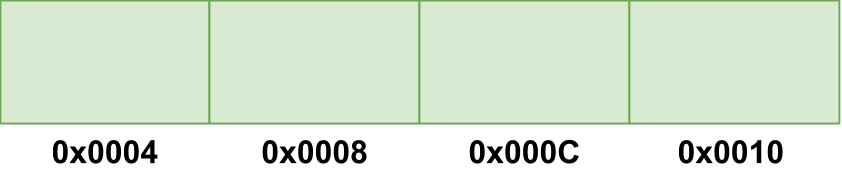
\includegraphics[width=1\textwidth]{memory}
\end{figure}


\begin{block}{}
	\begin{description}
		\item[stack] memory set aside for an execution thread (program)
		\item[heap] memory set aside for allocating on the fly
	\end{description}
\end{block}

\end{frame}




\begin{frame}{Declaration Statement}

	\begin{block}{How they're written:}
		\begin{center}
			\textcolor{DarkOrchid}{\textbf{type}} \textit{name};\\
			\pause
			\textcolor{DarkOrchid}{\textbf{type}} \textit{name1}, \textit{name2}, \textit{name3}, ...;
		\end{center}
	\end{block}
\end{frame}

\begin{frame}{Declaration Statement: Type}

\begin{figure}
	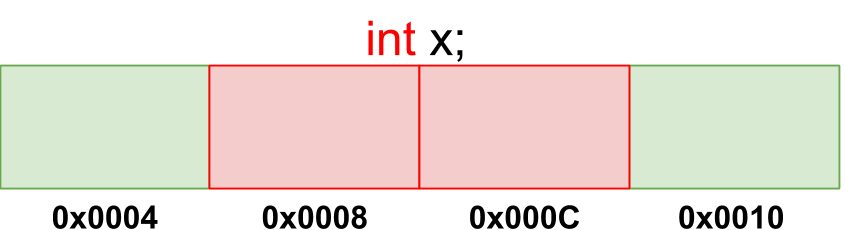
\includegraphics[width=1\textwidth]{dtype}
\end{figure}

\begin{block}{}
\begin{itemize}
	\item \textbf{type} allocates space in memory
	\item the primative types are: int, double, float, char, bool
	\item storage size can be specificed using: 
		\begin{itemize}
			\item long, short
			\item unsigned, signed
		\end{itemize}
\end{itemize}
\end{block}

\end{frame}

\begin{frame}{Declaration Statement: Variable Name}

\begin{figure}
	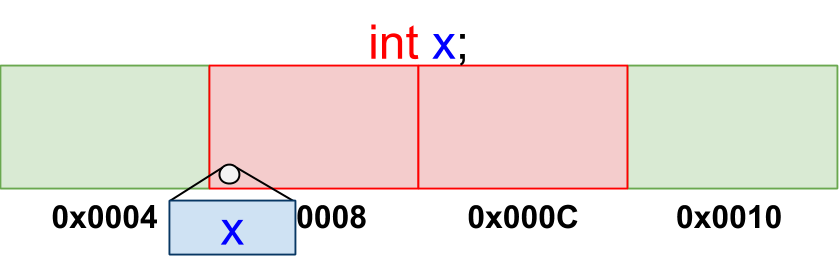
\includegraphics[width=1\textwidth]{label}
\end{figure}

\begin{block}{}
	\begin{itemize}
	 \item \textbf{name} labels space in memory
	\item \textbf{name} must follow the following rules:
		\begin{itemize}	
			\item First character has to be a letter or underscore
			\item Must be composed of letters, digits, and underscores
			\item Can't be part of the language	
		\end{itemize}
	\end{itemize}
\end{block}
\end{frame}

\begin{frame}{Initialization Statement: Value}

\begin{figure}
	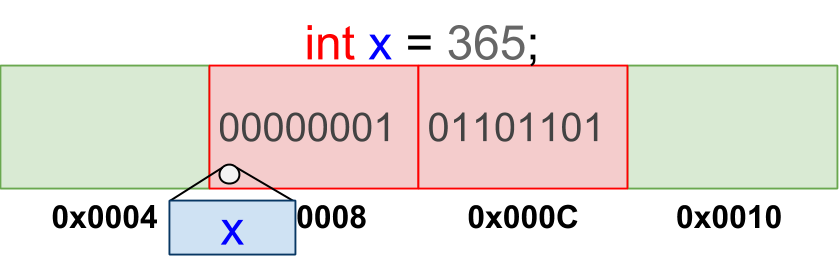
\includegraphics[width=1\textwidth]{init}
\end{figure}	

\begin{block}{}
	\begin{itemize}
		\item stores value in location identified by label
		\item value stored as binary number
	\end{itemize}
\end{block}
\end{frame}

\begin{frame}{Assignment Statement: Change}
\begin{figure}
	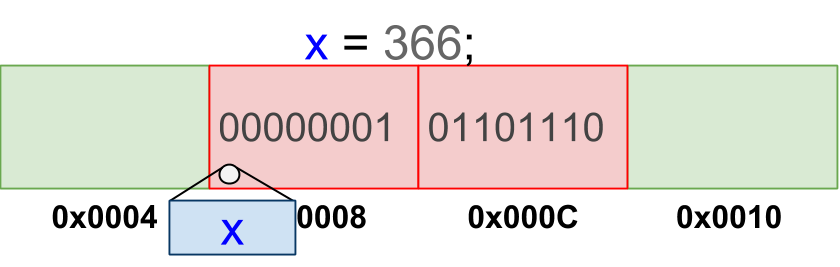
\includegraphics[width=1\textwidth]{change}
\end{figure}
\begin{block}{}
	\begin{itemize}
		\item stores value in location identified by label
		\item overwrites original value (if any)
	\end{itemize}
\end{block}
	
\end{frame}

\begin{frame}{Assignment Statement: Copy}
\begin{figure}
	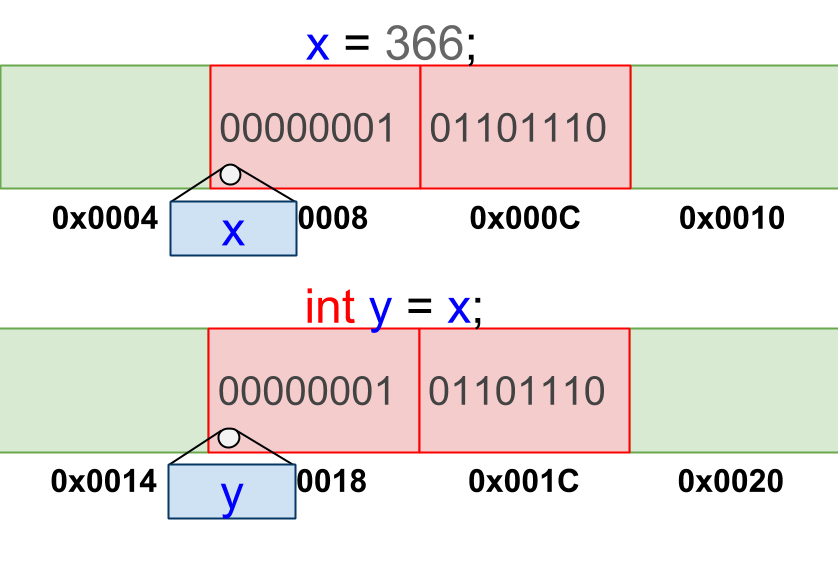
\includegraphics[width=1\textwidth]{copy}
\end{figure}
\end{frame}

\begin{frame}{Assignment Statement: Multiple Labels}
\begin{figure}
	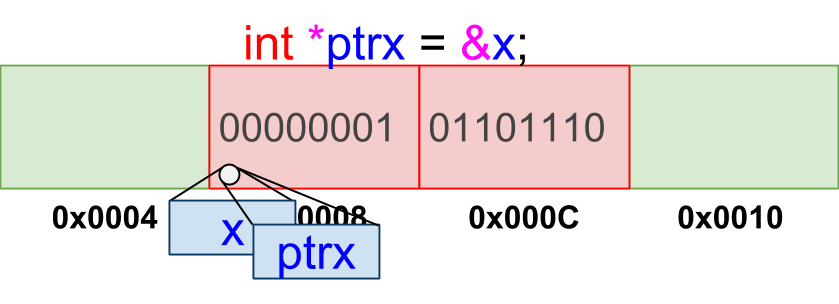
\includegraphics[width=1\textwidth]{ptr}
\end{figure}

\begin{block}{}
	\begin{description}
		\item[address operator \textbf{\&}] the address of the variable
		\item[indirection operator \textbf{*}] the value stored at that address		
	\end{description}
\end{block}
\end{frame}

\begin{frame}{Accumulators}
	\begin{block}{}
		\begin{itemize}
		\item used to keep track of subtotals
		\item operators: +=, -=, *=, /=, %=
		\end{itemize}
	\end{block}
	
	\begin{block}{}
		\begin{itemize}
			\item int sum = 10;
			\item sum = sum + 10;
			\item sum+=10;
		\end{itemize}
	\end{block}
\end{frame}

\begin{frame}{Counters}
\begin{block}{prefix}
	\begin{tabular}{l l}
		k=++n; & n = n+1; \\
			   & k = n;\\
	\end{tabular}
\end{block}
\begin{block}{postfix}
	\begin{tabular}{l l}
		k=n++; & k = n; \\
			   & n = n + 1;\\
	\end{tabular}
\end{block}
\end{frame}

\end{document}

